\documentclass{article}
\usepackage[utf8]{inputenc}
\usepackage{graphicx}
\usepackage{amsmath}
\usepackage{geometry}
\geometry{a4paper, margin=1in}
\usepackage{booktabs}
\usepackage{threeparttable}
\usepackage{tabularx}
\usepackage{array}
\usepackage{setspace}
\usepackage{parskip}
\usepackage{microtype}

% Load xcolor before hyperref to enable color definitions
\usepackage{xcolor}

% Configure hyperref for colored links instead of hidden links
\usepackage{hyperref}
\hypersetup{
    colorlinks=true,
    linkcolor=teal,      % Color for footnotes, equations, and cross-references
    citecolor=teal,      % Color for bibliography citations
    urlcolor=teal     % Color for external URLs
}

\usepackage{caption}
\captionsetup{font={small, color=black}, justification=centering}
\usepackage{fancyhdr}
\usepackage{float}
\usepackage{amssymb}
\usepackage{subcaption}
\usepackage{longtable}
\usepackage{multirow}
\usepackage[backend=biber, style=authoryear]{biblatex}
\addbibresource{references.bib}

% ---- Python / general code chunk design ----
% --------------------------------------------
\usepackage{listings}

\definecolor{code_comment}{RGB}{128, 128, 128}
\definecolor{code_keyword}{RGB}{0, 0, 204}
\definecolor{code_string}{RGB}{153, 0, 0}
\definecolor{code_bg}{RGB}{245, 245, 245}

\lstdefinestyle{pythonstyle}{
  backgroundcolor  = \color{code_bg},
  basicstyle       = \ttfamily\small,
  keywordstyle     = \color{code_keyword}\bfseries,
  commentstyle     = \color{code_comment}\itshape,
  stringstyle      = \color{code_string},
  numbers          = left,
  numberstyle      = \tiny\color{gray},
  stepnumber       = 1,
  breaklines       = true,
  frame            = single,
  language         = Python
}
\lstset{style=pythonstyle}
% --------------------------------------------
% --------------------------------------------

\newcolumntype{Y}{>{\centering\arraybackslash}X}
\setstretch{1.15}

\pagestyle{fancy}

\fancyhf{}
\rhead{\small CASA0011 --- Building and Describing an ABM}
\cfoot{\small\thepage}
\renewcommand{\headrulewidth}{0.4pt}

\title{
    \vspace{1cm}
    \Huge \textbf{Agent-Based Modelling --- Coursework 2} \\[0.5cm]
    \large CASA0011 --- Building and Describing an ABM\\[0.5cm]
    \Large \textit{Evaluating the Impact of Heterogeneous Cruising Strategies on\\ Urban Congestion: An Agent-Based Model of Midtown Manhattan} \\[1.5cm]
    
    
\includegraphics[width=0.85\textwidth]{cover.jpg} \\[0.5cm]
}

\author{
    \Large \textbf{Zhengpei Xu} \\[0.3cm]
    \large Student Number: 25034404 \\[0.3cm]
    \large \href{https://github.com/zhengpei-xu/CASA/blob/main/CASA0011_Agent-based-Modelling-for-Spatial-Systems/Coursework-2_Building-and-Describing-an-ABM/Model/ViscoCruise-Manhattan.nlogox}{Model Repository} \\[0.3cm]
}

\date{
    \vfill
    \large April 2026 \\[0.3cm]
    \normalsize Word Count: 1056
}

\begin{document}
\maketitle
\thispagestyle{empty}
\newpage
\pagenumbering{arabic}

% ============================================================
% 1. PARTIAL ODD DESCRIPTION
% ============================================================
\section{Partial ODD Description}

% ------------------------------------------------------------
% 1.1 PURPOSE AND PATTERNS
% ------------------------------------------------------------
\subsection{Purpose and Patterns}

% TODO: Research question(s) with question marks
% TODO: What patterns the model is designed to reproduce or explore
% TODO: Brief mention of relevant empirical patterns

This model investigates the following research question: How do the distinct vacant-cruising behaviours of taxis and for-hire vehicles\footnote{For-hire vehicles are henceforth referred to as FHVs in this text.} (e.g. Uber, Lyft) differentially contribute to traffic congestion within Midtown Manhattan's CBD?

\noindent Taxi drivers’ vacant-cruising strategy is rooted in local spatial experience, where they deliberately head for and slow down in high-demand zones to scan the kerbside for passengers. In contrast, FHV drivers primarily navigate under platform allocation mechanisms with more direct trajectories \parencite{millard-ball2023}. Based on this, the validity of this model can be verified through the following patterns:

\begin{itemize}
    \item \textbf{Strategic Clustering:}
    Taxis manifest intense spatial clustering in high-demand zones due to strategic cruising, whereas FHVs maintain a stochastic, uniform distribution, validating the emergent impact of heterogeneous cruising strategies.

    \item \textbf{Asymmetric Congestion Sensitivity:}
    As total vehicle number increases, average network speed should decrease. Moreover, increasing the number of taxis should disproportionately reduce average system speed relative to an equivalent increase in FHVs.
    
    \item \textbf{Demand-Efficiency Coupling:}
    Increased pickup demand should reduce competitive cruising and raise global-average-speed as agents transition from low-speed cruising to full-speed delivery.
\end{itemize}

% ------------------------------------------------------------
% 1.2 ENTITIES, STATE VARIABLES, AND SCALES
% ------------------------------------------------------------
\subsection{Entities, State Variables, and Scales}

% TODO: Introductory sentence

The model consists of three primary entities: Vehicles (background traffic, taxis, and FHVs), Passengers (pickup demand), and Patches (Manhattan grid topology). Global variables monitor aggregate performance.

Agent behaviours are driven by \texttt{vehicle-type} and \texttt{has-passenger?} status. Patch-level variables, including \texttt{demand-intensity} and directional flags, enforce the street system and dictate cruising logic. All vehicles incorporate a \texttt{reaction-delay} to simulate startup inertia and congestion recovery. A complete list of state variables is provided in Table~\ref{tab:entities}.

The world spans 121 × 78 square cells (with the origin (0,0) representing Times Square), each 10 m × 10 m in size, simulating the most congested part of Midtown Manhattan. Eight north-south avenue pairs (from 10th to Park Ave) and twelve east-west streets (from 50th to 39th Street) form the grid. The model uses a bounded, non-toroidal space to prevent ``wrap-around'' shortcuts.\footnote{The bounded space forces agents to use greedy navigation within the realistic grid constraints when delivering passengers.} Each tick represents one second in the real world.\footnote{While each tick represents one second, the traffic signal cycle is shortened to ~5 seconds (vs. real-world 45–90s) to prevent artificial gridlock at corners caused by the model's limited spatial extent.} Global variables track cumulative dead miles by vehicle type, trip counts, and speed metrics.



\begin{table}[H]
\begin{threeparttable}
\centering
\caption{Entities and State Variables}
\label{tab:entities}
\small 
\begin{tabularx}{\textwidth}{l l c X}
\toprule
\textbf{Entity} & \textbf{Variable} & \textbf{Type} & \textbf{Description} \\
\midrule
\multirow{7}{*}{\textbf{Vehicles}} 
  & \texttt{vehicle-type} & string & ``taxi''(yellow), ``FHV''(cyan), or ``background traffic''(blue) \\
  & \texttt{has-passenger?} & bool & Status flag (cruising phase or delivery phase(red)) \\
  & \texttt{target-patch} & patch & Destination for delivery \\
  & \texttt{is-congested?} & bool & Movement blocked by vehicle immediately ahead \\
  & \texttt{blocked-by-signal?} & bool & Blocked by red light at intersection boundaries \\
  & \texttt{did-move?} & bool & Binary flag for calculating instantaneous speed \\
  & \texttt{reaction-delay} & int & Stochastic recovery timer (1--2\,ticks) simulating startup inertia \\
\midrule
\textbf{Passengers} 
  & \texttt{destination-patch} & patch & Assigned trip endpoint on non-intersection road \\
\midrule
\multirow{6}{*}{\textbf{Patches}} 
  & \texttt{is-road?/is-intersection?} & bool & Grid topology: road vs.\ intersection classification \\
  & \texttt{is-signal-here?} & bool & Traffic light presence at intersection approaches \\
  & \texttt{is-green?} & bool & Current signal state of each signal patch \\
  & \texttt{can-go-N/S/E/W?} & bool & Hard constraints defining Manhattan's one-way system \\
  & \texttt{demand-intensity} & float & Calibrated from TLC pickup density (Jan 2025): 1.0 (High, 6th--Park Ave), 0.5 (Mid, 8th--6th Ave), 0.2 (Low, peripheral); drives passenger spawning and taxi cruising viscosity \\
\midrule
\multirow{12}{*}{\textbf{Global}} 
  & \multicolumn{3}{l}{\textit{Interface parameters (sliders)}} \\
  & \texttt{num-cars} & int & Total vehicle population \\
  & \texttt{commercial-vehicle-ratio} & float & Share of taxis + FHVs in total fleet \\
  & \texttt{Taxi-vs-FHV-split} & float & Proportion of taxis within commercial vehicles \\
  & \texttt{length-of-green-light} & int & Signal phase duration in ticks \\
  & \texttt{max-passengers} & int & System-wide passenger cap \\[4pt]
  & \multicolumn{3}{l}{\textit{Runtime state and metrics}} \\
  & \texttt{row-green?/col-green?} & bool & Current signal phase for E--W streets and N--S avenues \\
  & \texttt{taxi/FHV-dead-miles} & int & Cumulative search distance per vehicle type \\
  & \texttt{taxi/FHV-trips} & int & Cumulative completed passenger deliveries \\
  & \texttt{avg-dead-per-trip} & float & Operational efficiency metric per vehicle type \\
  & \texttt{global-avg-speed} & float & System-wide flow efficiency (ratio of moving agents) \\
  & \texttt{baseline-speed-value} & float & Pre-calculated reference speed for background-only traffic \\
\bottomrule
\end{tabularx}
\begin{tablenotes}
\footnotesize
\item \textit{Note: All variables correspond to the NetLogo model implementation. ``FHV'' represents For-Hire Vehicles (app-based ride-hailing). Binary flags (\texttt{bool}) are used for real-time metric aggregation. Global metric accumulators (dead-miles, trips, avg-speed) provide the output indicators against which the expected patterns are validated.}
\end{tablenotes}
\end{threeparttable}
\end{table}

% TODO: Spatial scale description
% TODO: Temporal scale description


% ------------------------------------------------------------
% 1.3 PROCESS OVERVIEW AND SCHEDULING
% ------------------------------------------------------------
\subsection{Process Overview and Scheduling}

% TODO: Describe the sequence of actions per tick
% TODO: Optionally include a flowchart
% TODO: Explain ordering: manage-signals -> generate-demand -> ask vehicles [check-for-pickup, check-for-arrival, execute-motion-logic] -> update metrics




The model operates in discrete-time execution, with each tick proceeding through four synchronised phases (Figure~\ref{fig:flowchart}): environment update (signal switching and stochastic passenger spawning), agent decision-making (type-specific cruising for vacant vehicles, greedy routing for occupied ones), physical execution (probabilistic movement with occupancy-based blocking), and data logging. Execution order within each agent class is randomised.

% ------------------------------------------------------------
% 1.5 INITIALISATION
% ------------------------------------------------------------
\subsection{Initialisation}

% TODO: Describe setup procedure
% TODO: Grid construction (avenues, streets, one-way logic)
% TODO: Vehicle creation and type assignment (commercial-vehicle-ratio, taxi-vs-ridehail-split)
% TODO: Demand zone setup (high/mid/low intensity)
% TODO: Signal initialisation
% TODO: What is randomised

At $t=0$, the environment is initialised as a $121 \times 78$ grid. Patches are assigned road (including intersection) or building attributes, with road patches receiving directional flags to enforce Manhattan's one-way system and a demand-intensity value to drive passenger spawning and taxi cruising viscosity. A total of $N$ vehicles are randomly distributed across road patches, initialised in a vacant state (no passenger, 2-tick reaction delay\footnote{The initial 2-tick delay is a synchronisation buffer to stagger vehicle start-up at $t=0$, and should not be confused with the 1--2 tick \texttt{reaction-delay} dynamically set during congestion recovery (see Section~1.6).}). Traffic lights on north-south avenues are set to green. All global performance metrics are reset to zero.

\begin{figure}[htbp]
    \centering
    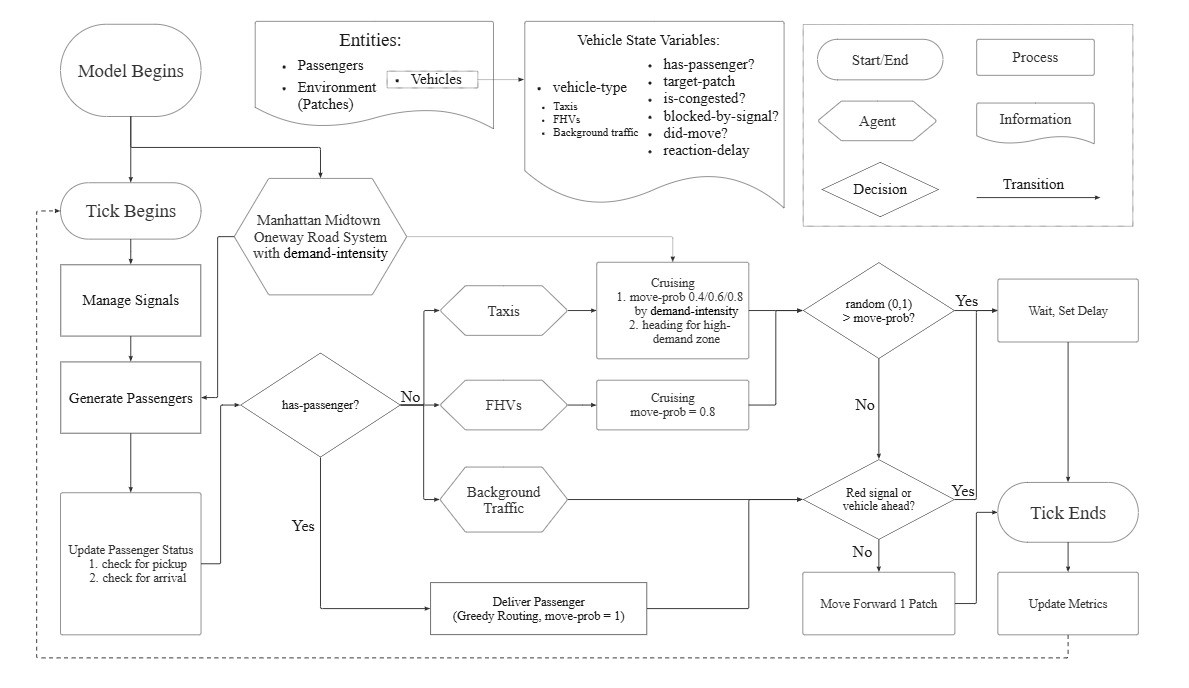
\includegraphics[width=\textwidth]{FlowChart.jpg}
    \caption{Process overview of the Visco-Cruise model}
    \label{fig:flowchart}
\end{figure}

% ------------------------------------------------------------
% 1.6 INPUT DATA
% ------------------------------------------------------------
\subsection{Input Data}

% TODO: State whether external data is used
% e.g. "The model does not use external input data to drive its dynamics. All demand patterns, network geometry, and agent parameters are generated internally during initialisation."
The model incorporates static spatial input derived from the TLC Trip Record Data. January 2025 yellow taxi trip records were filtered for evening rush hour (17:00--18:00) and aggregated by avenue corridor, producing three discrete \texttt{demand-intensity} tiers (1.0 / 0.5 / 0.2) that drive both stochastic passenger spawning and taxi cruising viscosity. The three-tier abstraction preserves the east-west demand gradient of Midtown while keeping the model computationally tractable (Figure~\ref{fig:demand_calibration}).



% ------------------------------------------------------------
% 1.7 SUBMODELS
% ------------------------------------------------------------
\subsection{Submodels}

% TODO: Full technical detail for each process
% - Signal management (manage-signals)
% - Passenger generation (generate-demand)
% - Motion logic (execute-motion-logic)
% - Taxi cruising direction (taxi-direction-report) -- 10-patch lookahead
% - Taxi speed modulation (taxi-speed-report) -- demand-dependent probability
% - Ride-hailing direction (ride-hailing-direction-report) -- random
% - Ride-hailing speed (ride-hailing-speed-report) -- fixed 0.8
% - Background traffic direction (background-traffic-direction-report) -- random
% - Delivery heading (decide-delivery-heading-report)
% - Pickup and arrival (check-for-pickup, check-for-arrival)

\textbf{Demand Spawning, Selection, and Delivery:} Every tick, passengers are stochastically generated on non-intersection road patches with probability proportional to \texttt{demand-intensity}, subject to a system-wide cap of \texttt{max-passengers}. When a vacant vehicle (taxi or FHV) occupies a patch holding a passenger, its state toggles to \texttt{has-passenger?~=~true} and a random \texttt{target-patch} is assigned. Occupied vehicles then use a greedy algorithm that minimises the Manhattan distance\footnote{Manhattan distance (or $L_1$ distance) between two points $(x_1, y_1)$ and $(x_2, y_2)$ is $|x_2 - x_1| + |y_2 - y_1|$, i.e. the travel distance along a rectangular grid. It is the natural metric for Manhattan's one-way street system, where diagonal movement is not permitted.} to their destination, subject to the one-way street constraints.

\textbf{Heterogeneous Cruising:} Vacant taxis scan a 10-patch radius ahead and rotate toward the heading with the highest cumulative \texttt{demand-intensity} with 80\% probability (20\% random exploration), and slow down in high-intensity zones ($\texttt{move-prob} = 0.4$, $0.6$, or $0.8$ depending on local demand), producing the cruising viscosity that gives the model its name. Vacant FHVs maintain undirected cruising at a constant $\texttt{move-prob} = 0.8$, reflecting passive platform dispatch. Background traffic moves randomly at full speed ($\texttt{move-prob} = 1.0$).

\textbf{Physical Congestion:} All movement is subject to occupancy-based blocking: if the patch ahead is occupied by another vehicle or controlled by a red signal, the vehicle stays stationary and resets its \texttt{reaction-delay} to a random value between 1 and 2 ticks, simulating human start-up inertia and triggering emergent shockwaves that propagate backward along the queue.

\begin{figure}[htbp]
    \centering
    \begin{subfigure}[b]{0.48\textwidth}
        \centering
        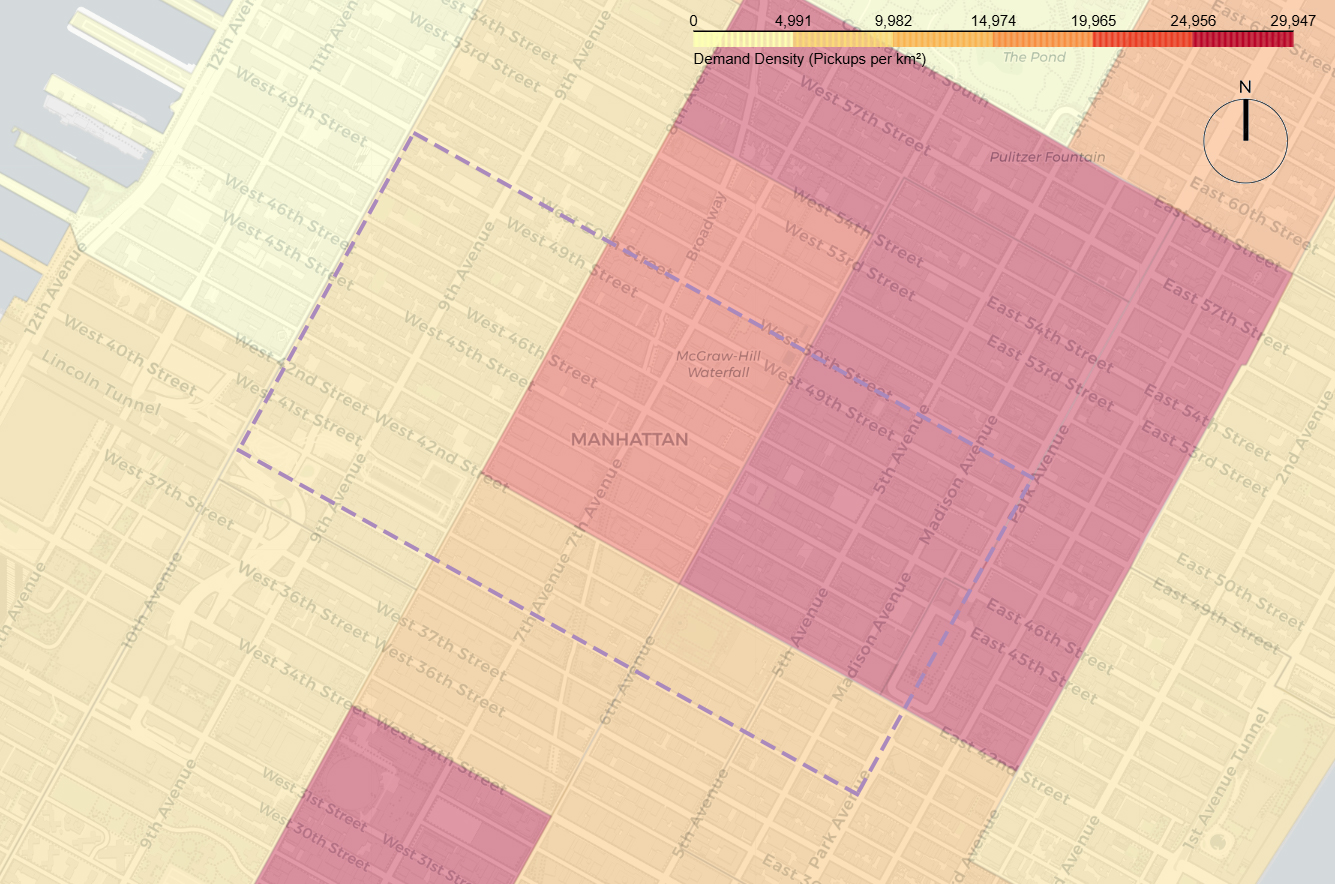
\includegraphics[height=5cm,keepaspectratio]{pickup-demand-heatmap.jpg}
        \caption{Yellow taxi pickup density, Jan 2025 evening rush hour. Purple dashed line indicates the modelled area.}
        \label{fig:demand_heatmap}
    \end{subfigure}
    \hfill
    \begin{subfigure}[b]{0.48\textwidth}
        \centering
        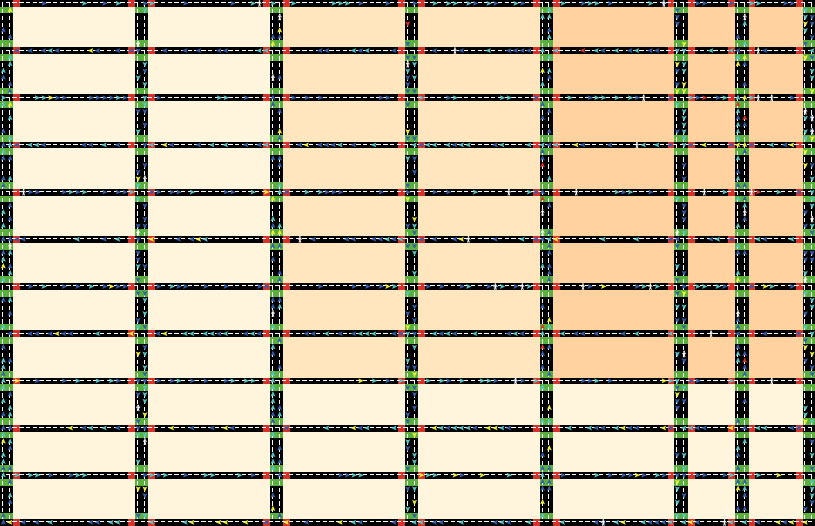
\includegraphics[height=5cm,keepaspectratio]{frame_001.png}
        \caption{Three-tier \texttt{demand-intensity} abstraction in the model (high / mid / low).}
        \label{fig:demand_model}
    \end{subfigure}
    \caption{Calibration of the \texttt{demand-intensity} field. Empirical TLC pickup density (a) is aggregated into three discrete tiers along the east-west gradient (b), capturing the strong concentration of demand between 6th Avenue and Park Avenue.}
    \label{fig:demand_calibration}
\end{figure}

% ============================================================
% 2. SITUATION OF MODEL WITHIN THE LITERATURE
% ============================================================
\section{Situation of Model Within the Literature}

% TODO: ~300-400 words
% Paragraph 1: Empirical context (congestion pricing, FHV deadheading problem)
% Paragraph 2: Existing ABM literature + gap + ABM justification
% Paragraph 3: ODD Design Concepts (Adaptation, Sensing, Emergence, Interaction, Stochasticity)
In January 2025, New York City introduced congestion pricing for its Central Business District, reducing vehicle entries by 11\% \parencite{cook2025}. \textcite{ostrovsky2024effective} show this reduction is driven predominantly by private vehicles. Taxis and FHVs, which are responsible for over 52\% of CBD traffic \parencite{tmrb2023} and unoccupied nearly half the time \parencite{cramer2016}, face lower per-trip charges and remain largely unaffected. \textcite{schaller2017} estimates that eliminating unnecessary cruising of taxis and FHVs could reduce total CBD VMT\footnote{Vehicle Miles Travelled: the total distance travelled by all vehicles in a given area over a specified period, a standard indicator of traffic output in US transport research.} by 7--11\%, highlighting vacant cruising as a significant lever for congestion relief. However, no established method adequately quantifies how these distinct cruising behaviours translate into localised congestion, making agent-based modelling a natural choice for its capacity to simulate individual driver decisions and capture their aggregate traffic impact.

Existing agent-based models have been applied to simulate taxi pickup-dropoff cycles and fleet efficiency \parencite{salanovagrau2013,ranjit2018}, and to assess the system-wide VMT impacts of autonomous vehicle rebalancing \parencite{fagnant2014,azevedo2020}. Neither strand models human-driven fleets with heterogeneous cruising strategies on a congested network. Building on the taxi pickup-dropoff paradigm, this Visco-Cruising model fills that gap by embedding distinct taxi and FHV cruising behaviours within a calibrated Manhattan grid and TLC demand data, revealing how bottom-up search strategies shape macro-level traffic and informing mixed-fleet policy decisions.

Following the ODD Design Concepts framework \parencite{grimm2020}, this model captures \textbf{adaptation} (taxis adjust cruising speed and heading in response to sensed local \texttt{demand-intensity}; FHVs maintain passive dispatch), \textbf{sensing} (taxis' 10-patch demand scanning behaviour), \textbf{interaction} (occupancy-based blocking by red signals or vehicles ahead), and \textbf{stochasticity} (TLC-calibrated passenger spawning). These micro-level behaviours produce \textbf{emergent} congestion and fleet-level dead-mile differentials, \textbf{observed} through system average speed, cumulative trips, and per-trip dead miles.

% ============================================================
% BIBLIOGRAPHY
% ============================================================
\newpage
\printbibliography

\end{document}

